\documentclass[fleqn]{jbook}
\usepackage{physpub}

\begin{document}

\begin{question}{専攻 問題1}{竹井洋(s91546)}
\parbox[t]{.5\linewidth}{
図1のような1次元ポテンシャル$V(x)$すなわち
\begin{eqnarray*}
V(x) &=& \infty \qquad \text{($\Norm{x}>d+a$のとき),} \\
V(x) &=& 0 \qquad \text{($d+a>\Norm{x}>d$のとき),} \\
V(x) &=& V_0 \qquad \text{($\Norm{x}<d$のとき),}
\end{eqnarray*}
の中に質量$m$の粒子が一個入っている系を考える。このように、1次元シュレディンガー方程式でポテンシャルエネルギーが1次元座標$x$の関数として$V(x)=V(-x)$を満たすとき、ハミルトニアン
\[ H(x)=-\frac{\hbar}{2m}\frac{\d{}^2}{\d{x}^2}+V(x) \]
}
\parbox[t]{.5\linewidth}{
\vspace*{-1cm}
\begin{center}
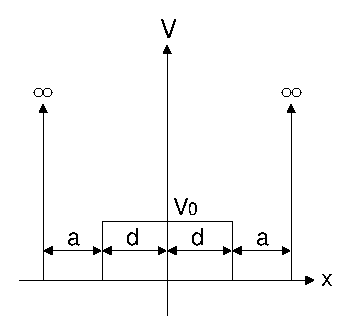
\includegraphics[clip]{1999phy1-1.eps}\\
図1
\end{center}
}
の固有関数$\Psi$は$\Psi(x)=\Psi(-x)$であるパリティが偶のものと$\Psi(x)=-\Psi(-x)$であるパリティが奇のものに分かれることに注意して、以下の問いに答えよ。但し$\hbar$はプランク定数である。


\begin{subquestions}

\SubQuestion

この系のエネルギー固有値$E$を決める式を$E<V_0$の条件が満たされている場合について求めよ。

\SubQuestion

基底状態と第一励起状態の波動関数をそれぞれ$\Ket{\Psi_0}$と$\Ket{\Psi_1}$とし、エネルギー固有値をそれぞれ$E=E_0,E_1$とする。$E_1<V_0$が満たされる場合に、$\Ket{\Psi_0}$と$\Ket{\Psi_1}$の概形を$x$の関数として描け。

\SubQuestion

$V_0$が有限で$d$が無限大の極限をとった時の$E_0,E_1$を$\overline{E_0},\overline{E_1}$とする。$\overline{E_0},\overline{E_1}$を一意的に決める式を求めよ。

\SubQuestion

$d$が大きいが有限であるとする。$\overline{E_0}$を用いて、$\Delta\equiv E_1-E_0$の$d$依存性がどうなっているかを議論せよ。
\end{subquestions}

$V_0$と$d$が大きいとき、規格化された波動関数$\Ket{\Psi_0}$や$\Ket{\Psi_1}$のほとんどの重みは$d+a>\Norm{x}>d$の中にあると考えてよい。したがって、$\Ket{\Psi_0}$や$\Ket{\Psi_1}$は近似的に右の井戸に粒子が存在し、わずかに$\Norm{x}<d$へ浸み出している状態$\Ket{R}$と、左の井戸に粒子が存在し、わずかに$\Norm{x}<d$へ浸み出している状態$\Ket{L}$の1次結合であらわされるとみなせる。$\Ket{R}$と$\Ket{L}$は規格化され、互いに直交しているとし、また、$\Ket{\Psi_0}$や$\Ket{\Psi_1}$よりも高い励起状態については無視して良いとして、以下に答えよ。

\begin{subquestions}[5]

\SubQuestion

$\Ket{\Psi_0}$と$\Ket{\Psi_1}$を$\Ket{R}$と$\Ket{L}$の1次結合で表せ。

\SubQuestion

$\Ket{R}$と$\Ket{L}$を基底とする表現をとって、ハミルトニアンを2行2列の行列で表せ。

\SubQuestion

$t=0$に粒子の波動関数が右の井戸に存在する状態$\Ket{R}$で表わされていたとき、トンネリングによって時刻$t$に粒子が左の井戸の状態$\Ket{L}$に移っている確率を$\Delta$を用いて表わし、得られた$\Delta$依存性の物理的意味を議論せよ。

\end{subquestions}
\end{question}
\begin{answer}{専攻 問題1}{竹井洋(s91546)}
\begin{subanswers}

\SubAnswer
$\Psi_{\pm}(x)=\pm\Psi_{\pm}(-x)$のような解がある。
\begin{itemize}
\item[(i)]
~$0\le x \le d$のとき

\begin{gather*}
-\frac{\hbar^2}{2m}\Psi_{1\pm}''(x)+V_0\Psi_{1\pm}(x)=E_{\pm}\Psi_{1\pm}(x) \\
\alpha_{\pm}\equiv\frac{\sqrt{2m(V_0-E_{\pm})}}{\hbar}\;  \text{として} \\
\Psi_{1\pm}(x)=Ae^{\alpha_{\pm} x}+Be^{-\alpha_{\pm} x} \\
\end{gather*}

\begin{itemize}

\item[\textbullet] ~parity evenのとき
\begin{gather*}
\Psi_{1+}(x)=\Psi_{1+}(-x)\; \text{より} \; A=B \\
\therefore \Psi_{1+}(x)=A_+\cosh (\alpha_+ x) \\
\end{gather*}

\item[\textbullet] ~parity oddのとき
\begin{gather*}
\Psi_{1-}(x)=-\Psi_{1-}(-x)\; \text{より} \; A=-B \\
\therefore \Psi_{1-}(x)=A_-\sinh (\alpha_- x) \\
\end{gather*}

\end{itemize}

\item[(ii)]
~$d\le x \le d+a$のとき
\begin{gather*}
-\frac{\hbar^2}{2m}\Psi_{2\pm}''(x)=E_{\pm}\Psi_{2\pm}(x) \\
\beta_{\pm}\equiv \frac{\sqrt{2mE_\pm}}{\hbar}\; \text{として}\\
\Psi_{2\pm}(d+a)=0\text{の境界条件より}\\
\Psi_{2\pm}(x)=B_{\pm}\sin\left(\beta_\pm(x-a-d)\right) \\
\text{と書ける。}
\end{gather*}

\end{itemize}
これらから$E$を求める。

\begin{itemize}

\item ~parity evenのとき

\begin{gather*}
\begin{cases}
\Psi_{1+}(x)=A_+\cosh\alpha_+x \\
\Psi_{2+}(x)=B_+\sin\left(\beta_+(x-a-d)\right)
\end{cases}
\\
\text{境界条件より}
\\
\begin{cases}
\Psi_{1+}(d)=\Psi_{2+}(d) \\
\Psi'_{1+}(d)=\Psi'_{2+}(d)
\end{cases}
\\
\text{したがって}
\\
\begin{cases}
A_+\cosh\alpha_+d=-B_+\sin\beta_+a \\
A_+\alpha_+\sinh\alpha_+d=B_+\beta_+\cos\beta_+a
\end{cases}
\\
\therefore \alpha_+\tanh\alpha_+d=-\beta_+\cot\beta_+a
\end{gather*}

これにより$E$が求まる。

\item ~parity oddのとき

\begin{gather*}
\begin{cases}
\Psi_{1-}(x)=A_-\sinh\alpha_-x \\
\Psi_{2-}(x)=B_-\sin\left(\beta_-(x-a-d)\right)
\end{cases}
\\
\text{境界条件より}
\\
\begin{cases}
\Psi_{1-}(d)=\Psi_{2-}(d) \\
\Psi'_{1-}(d)=\Psi'_{2-}(d)
\end{cases}
\\
\text{したがって}
\\
\begin{cases}
A_-\sinh\alpha_-d=-B_-\sin\beta_-a \\
A_-\alpha_-\cosh\alpha_-d=B_-\beta_-\cos\beta_-a
\end{cases}
\\
\therefore \frac{1}{\alpha_-}\tanh\alpha_-d=-\frac{1}{\beta_-}\tan\beta_-a
\end{gather*}

これにより$E$が求まる。

\end{itemize}

\SubAnswer

parity evenのとき。
\begin{center}
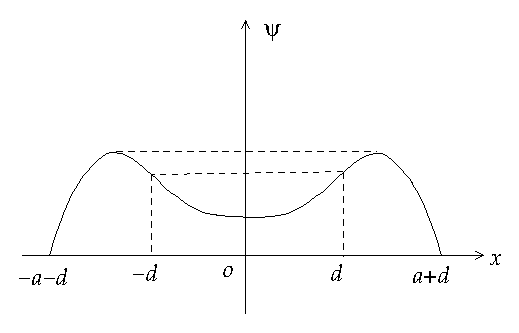
\includegraphics[clip]{1999phy1-2.eps}
\end{center}

parity oddのとき。
\begin{center}
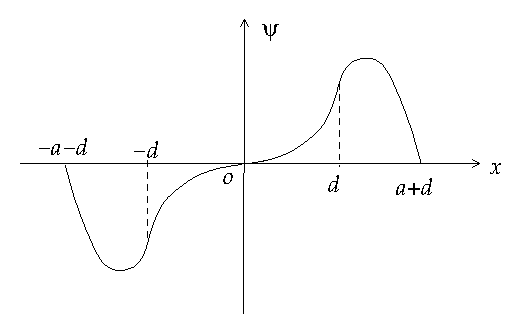
\includegraphics[clip]{1999phy1-3.eps}
\end{center}

\SubAnswer
$d\rightarrow\infty$では
\[ \tan\beta_{\pm}a=-\frac{\beta_{\pm}}{\alpha_{\pm}} \]
より、エネルギー準位は縮退していて
\[ \overline{E_0}=\overline{E_1} \]
エネルギーの値もこの式より求まる。

\SubAnswer

\begin{align*}
\tanh\alpha x &= \frac{e^{\alpha x}-e^{-\alpha x}}{e^{\alpha x}+e^{-\alpha x}} \\
&= \frac{1-e^{-2\alpha x}}{1+e^{-2\alpha x}}
\end{align*}
$x$が十分大きいとすると
\begin{align*}
\tanh\alpha x &\sim \left(1-e^{-2\alpha x}\right)^2 \\
&\sim 1-2e^{-2\alpha x}
\end{align*}
したがって
\[ \tan\beta_{\pm}a=-\frac{\beta_{\pm}}{\alpha_{\pm}}\mp 2\frac{\beta_{\pm}}{\alpha_{\pm}}e^{-2\alpha_{\pm}d} \]
\begin{gather*}
\alpha_0\equiv\frac{\sqrt{2m(V_0-E_0)}}{\hbar}\; ,\;\beta_0\equiv \frac{\sqrt{2mE_0}}{\hbar}\;\text{とすると}\\
\beta_{\pm}a=\pi-\frac{\beta_0}{\alpha_0}\left(1\pm2e^{-2\alpha_0 d}\right)
\end{gather*}

$\beta_+$は基底状態、$\beta_-$は第一励起状態となるので
\[ \Delta\equiv E_1-E_0=\frac{\hbar^2}{2m}\left(\beta_-^2-\beta_+^2\right) \quad \cdots \quad \propto e^{-2\alpha_0d} \]
よって、$\Delta$は$d$に指数関数的に依存している。

\SubAnswer

\begin{align*}
\Ket{\Psi_0}&=\frac{1}{\sqrt{2}}\Bigl( \Ket{R}+\Ket{L}\Bigr) \\
\Ket{\Psi_1}&=\frac{1}{\sqrt{2}}\Bigl( \Ket{R}-\Ket{L}\Bigr)
\end{align*}

\SubAnswer

\begin{align*}
\Ket{R}&=\frac{1}{\sqrt{2}}\Bigl( \Ket{\Psi_0}+\Ket{\Psi_1}\Bigr) \\
\Ket{L}&=\frac{1}{\sqrt{2}}\Bigl( \Ket{\Psi_0}-\Ket{\Psi_1}\Bigr)
\end{align*}

\begin{align*}
\Bracket{R}{H}{R} &= \frac{1}{2}\Bigl(\Bra{\Psi_0}+\Bra{\Psi_1}\Bigr)\Bigl(E_0\Ket{\Psi_0}+E_1\Ket{\Psi_1}\Bigr)
= \frac{E_0+E_1}{2} \\
\Bracket{L}{H}{L} &= \frac{1}{2}\Bigl(\Bra{\Psi_0}-\Bra{\Psi_1}\Bigr)\Bigl(E_0\Ket{\Psi_0}-E_1\Ket{\Psi_1}\Bigr)
= \frac{E_0+E_1}{2} \\
\Bracket{R}{H}{L} &= \frac{1}{2}\Bigl(\Bra{\Psi_0}+\Bra{\Psi_1}\Bigr)\Bigl(E_0\Ket{\Psi_0}-E_1\Ket{\Psi_1}\Bigr)
= -\frac{E_1-E_0}{2}
= -\frac{\Delta}{2} \\
\Bracket{L}{H}{R} &= \frac{1}{2}\Bigl(\Bra{\Psi_0}-\Bra{\Psi_1}\Bigr)\Bigl(E_0\Ket{\Psi_0}+E_1\Ket{\Psi_1}\Bigr)
= -\frac{E_1-E_0}{2}
= -\frac{\Delta}{2} \\
\end{align*}
\[ 
\therefore H \doteq
\begin{pmatrix}
\cfrac{E_0+E_1}{2} & -\cfrac{\Delta}{2} \\
-\cfrac{\Delta}{2} & \cfrac{E_0+E_1}{2}
\end{pmatrix}
\]
\\


\SubSubAnswer
Schr\"{o}dinger表示で考える。

\begin{gather*}
H\Ket{R(t)}=i\hbar\frac{\del}{\del t}\Ket{R(t)}\; ,\; \Ket{R(0)}=\Ket{R} \\
\therefore \Ket{R(t)}=e^{-iHt/\hbar}\Ket{R}
\end{gather*}

\begin{align*}
e^{-iHt/\hbar} &\doteq \sum_k\frac{(-it/\hbar)^k}{k!}
\begin{pmatrix}
\frac{E_0+E_1}{2} & -\frac{\Delta}{2} \\
-\frac{\Delta}{2} & \frac{E_0+E_1}{2}
\end{pmatrix}
^k \\
&= \sum_k\frac{1}{k!}\frac{(-it/\hbar)^k}{2}
\begin{pmatrix}
E_0^k+E_1^k & E_0^k-E_1^k \\
E_0^k-E_1^k & E_0^k+E_1^k 
\end{pmatrix}
\\
&= \frac{1}{2}
\begin{pmatrix}
e^{-iE_0t/\hbar}+e^{-iE_1t/\hbar} & e^{-iE_0t/\hbar}-e^{-iE_1t/\hbar} \\
e^{-iE_0t/\hbar}-e^{-iE_1t/\hbar} & e^{-iE_0t/\hbar}+e^{-iE_1t/\hbar}
\end{pmatrix}
\end{align*}

\begin{align*}
\therefore \Product{L}{R(t)} &= \frac{1}{2}\Bra{L}\left\{ \left(e^{-iE_0t/\hbar}+e^{-iE_1t/\hbar}\right)\Ket{R}+\left(e^{-iE_0t/\hbar}-e^{-iE_1t/\hbar}\right)\Ket{L}\right\} \\
&= \frac{1}{2}\left(e^{-iE_0t/\hbar}-e^{-iE_1t/\hbar}\right)
\end{align*}

\begin{align*}
\therefore \Norm{\Product{L}{R(t)}}^2 &= \frac{1}{4}\left(e^{-iE_0 t/\hbar} - e^{-iE_1 t/\hbar}\right)
\left(e^{iE_0 t/\hbar} - e^{iE_1 t/\hbar}\right)\\
&= \frac{1}{4}\left(2-e^{-i\Delta t/\hbar}-e^{i\Delta t/\hbar}\right)\\
&= \frac{1}{2}\left(1-\cos\frac{\Delta}{\hbar}t \right)\\
&=\sin^2\frac{\Delta}{2\hbar}t
\end{align*}

これより、$\Delta$が大きい、つまり$V_0$や$d$が小さい時ほど速く$\Ket{R}\leftrightarrow\Ket{L}$の周期的遷移をすることがわかる。

\end{subanswers}
\end{answer}


\end{document}
